\documentclass[12pt]{article}

\usepackage{amsmath}        % Matrice
\usepackage{amsfonts}       % Math font
\usepackage[french]{babel}  % Alinea
\usepackage{float}          % Position image
\usepackage[T1]{fontenc}    %
\usepackage{geometry}       % Layout
\usepackage{graphicx}       % Image
\usepackage{titling}        % Title
\usepackage{fancyhdr}       % Header

\title{Algorithmique et Complexité : TP1}
\author{MÉTAYER Stevan \break GEFFROY Noam}
\date{\today}

% Header
\setlength{\headheight}{52pt}
\pagestyle{fancy}
\fancyhead{}
\fancyhead[R]{\thetitle}
% \fancyhead[L]{}

\allowdisplaybreaks

\newcommand*{\addheight}[2][.5ex]{%
  \raisebox{0pt}[\dimexpr\height+(#1)\relax]{#2}%
}

\begin{document}

% Premiere page
\begin{titlepage}

% Logo
\begin{figure}
    
\includegraphics[width=12em]{esir.png}
    \hfill
    
\includegraphics[width=12em]{ur.png}
    \label{fig:logos}
\end{figure}

% Titre
\vspace*{5cm}
\begin{center}\rule{\linewidth}{2pt}\end{center}
\begin{center}  
\large \textbf{{\huge \thetitle} }
\rule \linewidth{2pt}
\end{center}

% Auteur(s)
\begin{center} {\large \textbf{{\large \theauthor}}} \end{center}
\vspace{\fill}
\begin{flushright}
    \large \today
    \vspace*{-3.5cm}
\end{flushright}

\end{titlepage}


% Sommaire
\newpage

\renewcommand*\contentsname{Sommaire}
\setcounter{tocdepth}{3}
\tableofcontents

\newpage

\section{Analyse de tris}

\subsection{Tri par insertion}

On étudie la complexité de l'algorithme de tri par insertion en fonction des différents cas possibles :
\newline

\begin{tabular}[H]{c c}
    \addheight{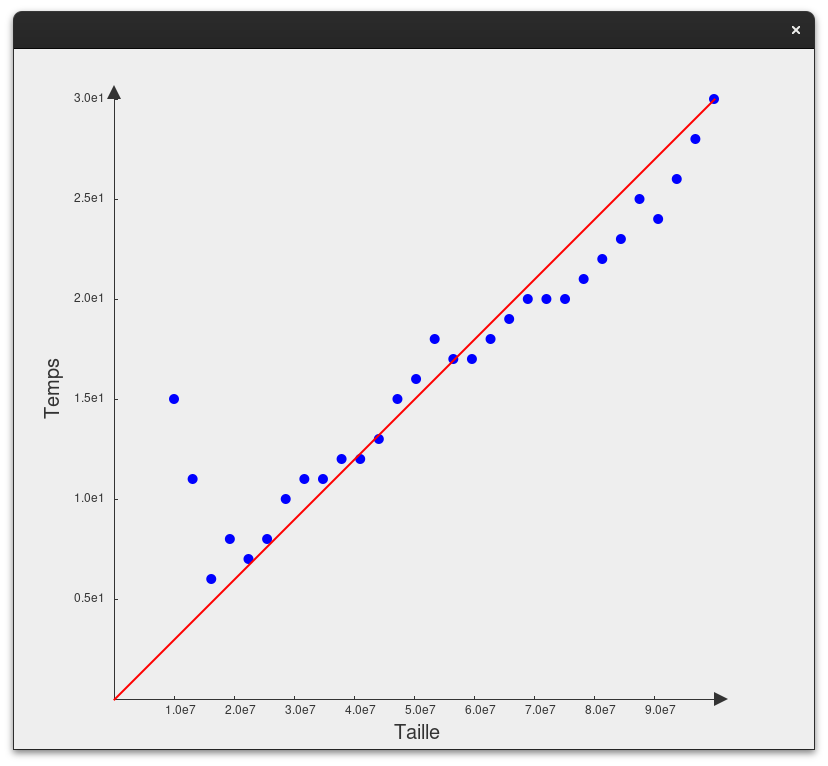
\includegraphics[width=18em]{ins_meilleur.png}} &
    \addheight{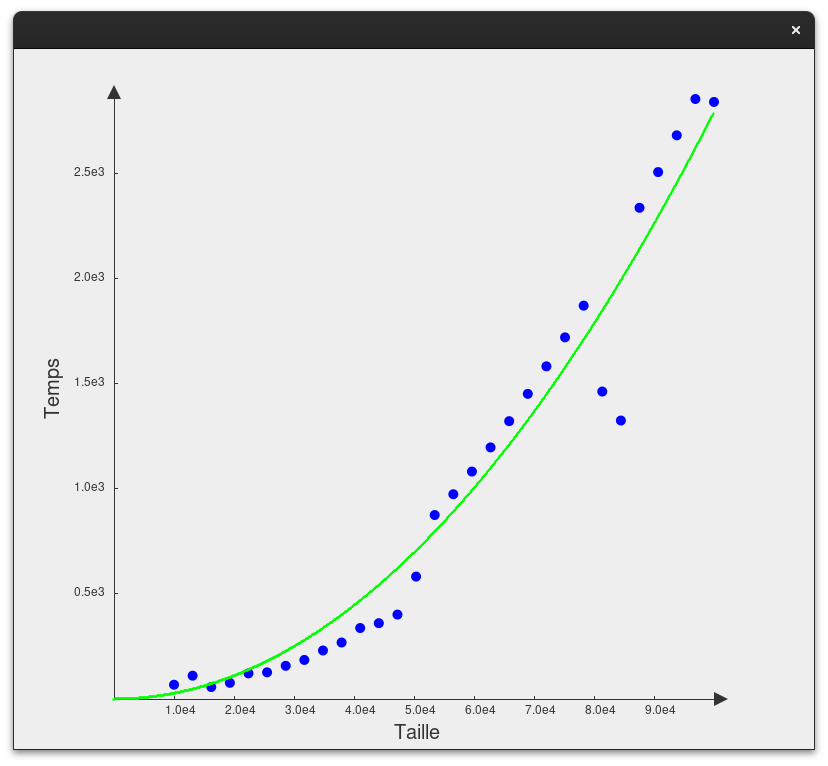
\includegraphics[width=18em]{ins_pire.png}} \\
    \small \textbf{Meilleur cas} & \textbf{Pire cas} \\
    \addheight{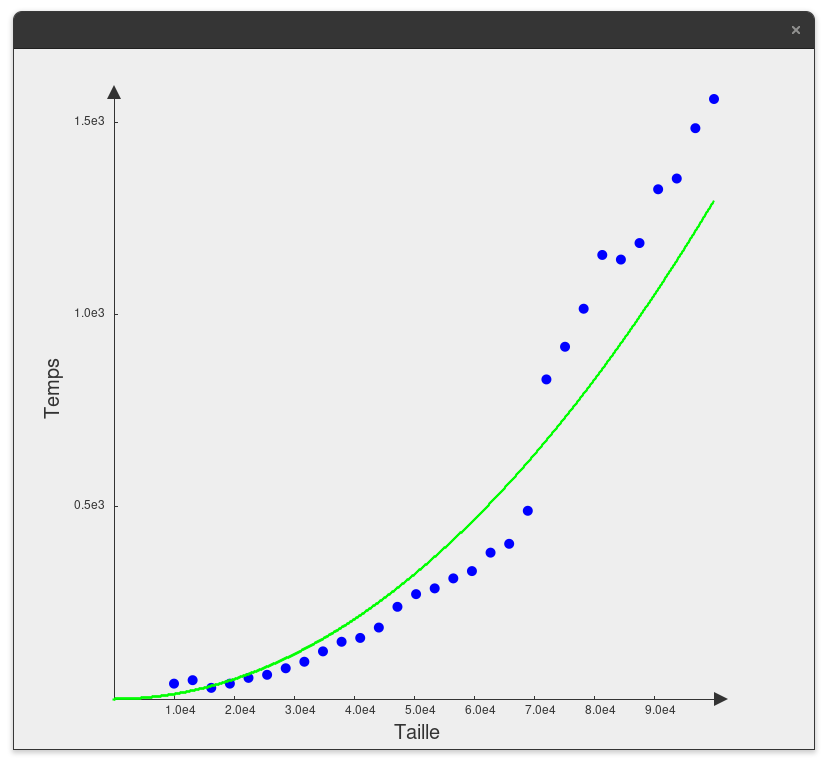
\includegraphics[width=18em]{ins_gen.png}}  & \\
    \small \textbf{Cas général} & \\
\end{tabular}


On trouve des complexités différentes en fonction des différents cas. Dans le meilleur cas, c'est-à-dire quand le tableau est déjà trié, l'algorithme possède une complexité linéaire. Dans le pire cas (tableau trié en sens inverse) et le cas général, l'algorithme passe en complexité quadratique. Le coefficient quadratique dans le cas général est égal à $1.3*10^{-7}$ dans notre cas.

\subsubsection*{Étude sur la population française}

On regarde ensuite le temps estimé de l'algorithme avec un tableau de 67 millions d'éléments.
On utilise le coefficient trouvé dans le cas général du tri par insertion.
$ t = 13*10^{-8} * 67*10^6 = 583570000 $ secondes. Ce qui équivaut à 6 jours 18 heures 6 minutes 10 secondes.

\subsection{Tri fusion}

On étudie la complexité de l'algorithme de tri fusion uniquement dans le cas général :

\begin{tabular}[H]{c c}
    \addheight{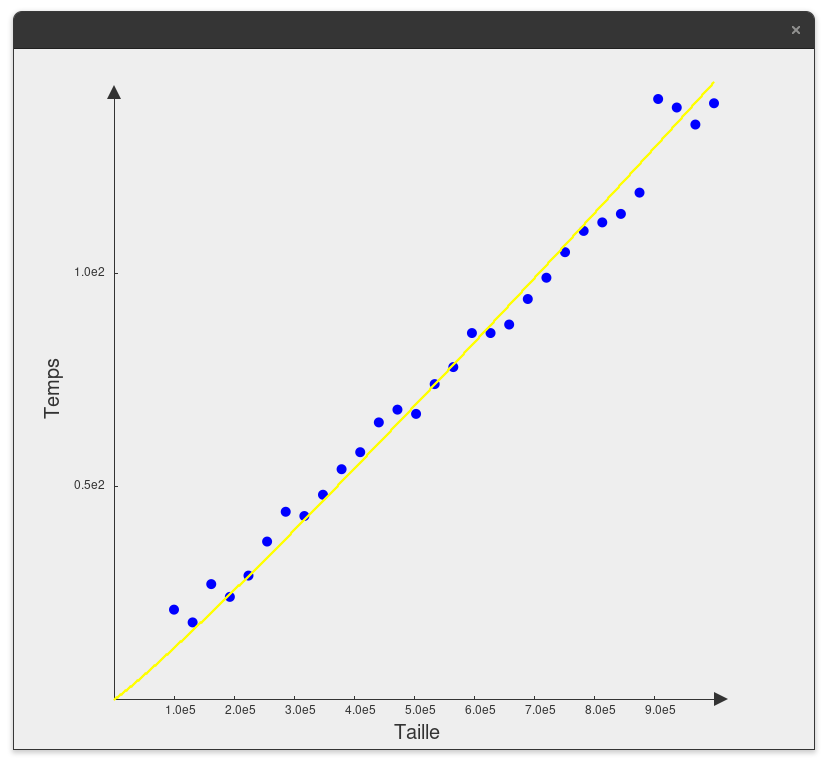
\includegraphics[width=18em]{fus_gen.png}}  & \\
    \small \textbf{Cas général} & \\
\end{tabular}

L'algorithme possède une complexité en $n log(n)$. La courbe du temps d'exécution en fonction de la taille du tableau obtenue est similaire à une courbe linéaire.
Le coefficient de la droite est environ égal à $1.05*10^{-5}$ dans notre cas.

\subsubsection*{Étude sur la population française}

On étudie de nouveau le temps d'exécution de l'algorithme sur la population française.
On utilise le coefficient de la droite trouvé dans le cas général pour estimer le temps d'exécution. $ t = 1.05*10^{-5} * 67*10^6 = 703 $ secondes. Ce qui équivaut à 8 minutes 23 secondes.

\subsubsection*{Conclusion}

On peut en conclure que l'algorithme de tri fusion est meilleur que le tri par insertion dans le cas général. L'efficacité du tri fusion est surtout remarquable dans le cas de grands tableaux à trier où l'on peut passer d'un temps d'exécution d'une semaine à seulement quelques minutes.


\section{Permutations}

On s'intéresse ensuite aux permutations.
La fonction fournie effectue des permutations sur une chaine de caractères avec les lettres de l'alphabet en faisant toutes les combinaisons possibles d'ordre.
En supposant que la complexité est du même ordre de grandeur que le nombre d'affichages réalisés, il y existe n factoriel combinaisons pour une chaine de caractères. La complexité est donc $n!$.


On affiche l'évolution du temps de calcul en fonction de n, la taille de la chaine de caractères :

\begin{tabular}[H]{c c}
    \addheight{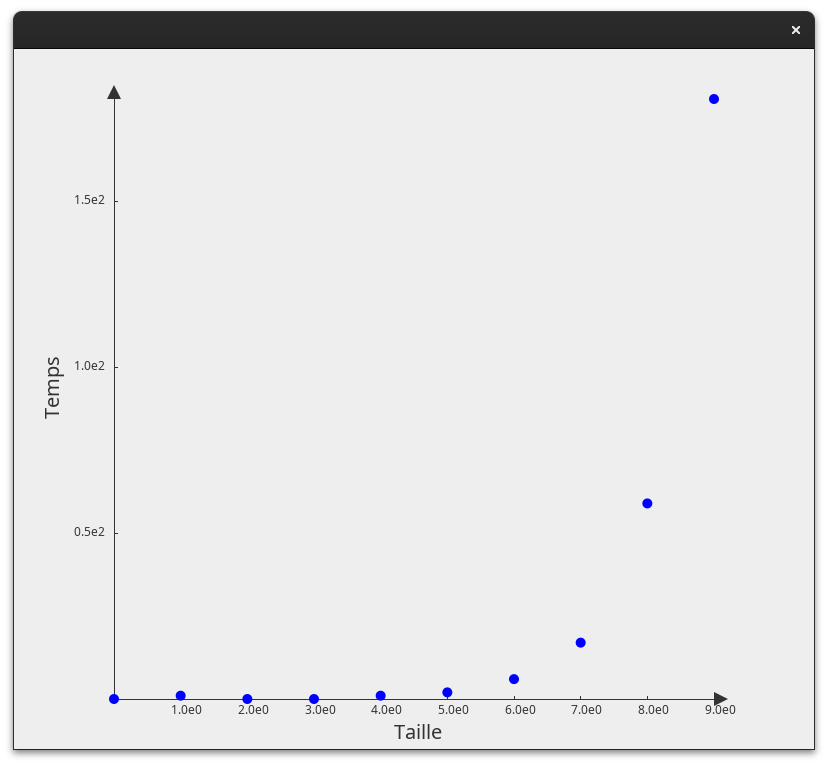
\includegraphics[width=18em]{permu.png}}  & \\
    \small \textbf{Permutation} & \\
\end{tabular}

En se servant de la courbe obtenue on peut estimer le temps d'exécution pour $n=26$. On trouve $2.1*10^12$ ans, ce qui est plus grand que l'âge de l'univers.


\end{document}